% ------------------------------------------------------------------------------
% TYPO3 Version 10.1 - What's New (Italian Version)
%
% @license	Creative Commons BY-NC-SA 3.0
% @link		http://typo3.org/download/release-notes/whats-new/
% @language	Italian
% ------------------------------------------------------------------------------

\section{Modifiche per integratori}
\begin{frame}[fragile]
	\frametitle{Modifiche per integratori}

	\begin{center}\huge{Capitolo 2:}\end{center}
	\begin{center}\huge{\color{typo3darkgrey}\textbf{Modifiche per integratori}}\end{center}

\end{frame}

% ------------------------------------------------------------------------------
% Feature | 89102 | Read settings for sites from <config>/sites/<siteIdentifier>/settings.yaml
%
%\begin{frame}[fragile]
%	\frametitle{Changes for Integrators}
%	\framesubtitle{Site-specific Settings (1)}
%
%	% decrease font size for code listing
%	\lstset{basicstyle=\smaller\ttfamily}
%
%	\begin{itemize}
%		\item A YAML file can provide site specific variables independent of the current context.
%
%		\item Place the file in the site configuration folder:\newline
%			\texttt{<config>/sites/<siteIdentifier>/settings.yaml}
%
%		\item For example:
%
%\begin{lstlisting}
%Vendor:
%   MyExtension:
%      storagePid: 1
%      limit: 15
%\end{lstlisting}
%
%	\end{itemize}
%
%\end{frame}
%
% ------------------------------------------------------------------------------
% Feature | 89102 | Read settings for sites from <config>/sites/<siteIdentifier>/settings.yaml
%
%\begin{frame}[fragile]
%	\frametitle{Changes for Integrators}
%	\framesubtitle{Site-specific Settings (2)}
%
%	% decrease font size for code listing
%	\lstset{basicstyle=\smaller\ttfamily}
%
%	\begin{itemize}
%		\item Settings can be accessed in TypoScript:
%
%\begin{lstlisting}
%plugin.tx_example.storagePid = {$Vendor.MyExtension.storagePid}
%\end{lstlisting}
%
%		\item Settings can also be accessed in PHP using the \texttt{Site} object:
%
%\begin{lstlisting}
%$settings = $site->getSettings();
%$storagePid = $settings['MyVendor']['MyExtension']['storagePid'];
%\end{lstlisting}
%
%	\end{itemize}
%
%\end{frame}

% ------------------------------------------------------------------------------
% Feature | 89227 | Ask for email address while installing TYPO3

\begin{frame}[fragile]
	\frametitle{Modifiche per integratori}
	\framesubtitle{Indirizzo email dell'Amministratore}

	\begin{columns}[T]
		\begin{column}{.04\textwidth}
		\end{column}
		\begin{column}{.38\textwidth}

			Un indirizzo email può essere inserito nel processo di installazione.
			Questo indirizzo è utilizzato per l'utente amministratore iniziale del backend.
			\vspace{0.2cm}

			La stessa opzione esiste nel modulo di manutenzione dell'Install Tool
			\textbf{Crea utente amministratore}.

		\end{column}
		\begin{column}{.58\textwidth}
			\vspace{-0.3cm}
			\begin{figure}
				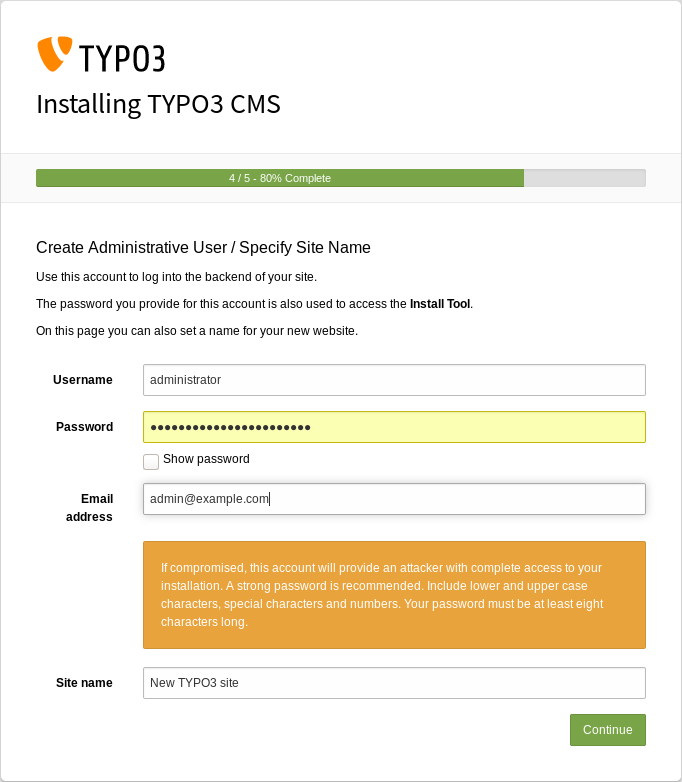
\includegraphics[width=0.70\linewidth]{ChangesForIntegrators/89227-EmailAddressDuringInstallation.png}
			\end{figure}
		\end{column}
	\end{columns}

\end{frame}

% ------------------------------------------------------------------------------
% Feature | 89229 | Cache Preset for Settings in Maintenance Area

% TRANSLATORS, PLEASE BE AWARE:
% We already included this slide in the 10.0 What's New Slides! However, the
% feature #89229 was removed from the TYPO3 core shortly before version 10.0 was
% published. Therefore, you possibly don't need to translate this slide again
% (just copy the text from the previous What's New Slides (search for the term
% "Cache Storage Type" in file ChangesForIntegrators.tex).

\begin{frame}[fragile]
	\frametitle{Modifiche per integratori}
	\framesubtitle{Tipo di archiviazione della Cache (1)}

	\begin{itemize}

		\item TYPO3 presenta un sistema di memorizzazione nella cache flessibile, con una
		    configurazione predefinita che è l'ideale per la maggior parte dei casi d'uso.
		\item Ora è possibile configurare il tipo di archiviazione per ottimizzare la cache
		    e aumentare le prestazioni in base al singolo ambiente.

			\begin{itemize}
				\item Scegli l'archivio \textbf{database} per un ambiente standard o se ad
					esempio viene utilizzato un file system di rete (NFS).
				\item Scegli \textbf{file system} se, ad esempio, viene utilizzata un'installazione
				    di database distribuita.
				\item Scegli \textbf{impostazioni della cache personalizzate} per configurare il tipo
				    di archiviazione per ogni cache in modo indipendente.
			\end{itemize}

		\item Per installazioni più complesse, dovrebbero essere considerate cache memory-based come
			\href{https://redis.io/}{Redis}
			o
			\href{https://memcached.org/}{Memcached}.

	\end{itemize}

\end{frame}

% ------------------------------------------------------------------------------
% Feature | 89229 | Cache Preset for Settings in Maintenance Area

% TRANSLATORS, PLEASE BE AWARE:
% We already included this slide in the 10.0 What's New Slides! However, the
% feature #89229 was removed from the TYPO3 core shortly before version 10.0 was
% published.
%
% On this slide, the path to the function in the backend needs to be adjusted:
% ADMIN TOOLS -> Settings -> Configuration Presets

\begin{frame}[fragile]
	\frametitle{Modifiche per integratori}
	\framesubtitle{Tipo di archiviazione della Cache (2)}

	\begin{itemize}

		\item Backend: \textbf{MAINTENANCE} \ding{223}\hspace{0.1cm}\textbf{Settings} \ding{223}\hspace{0.1cm}\textbf{Cache}:
		\end{itemize}

	\begin{figure}
		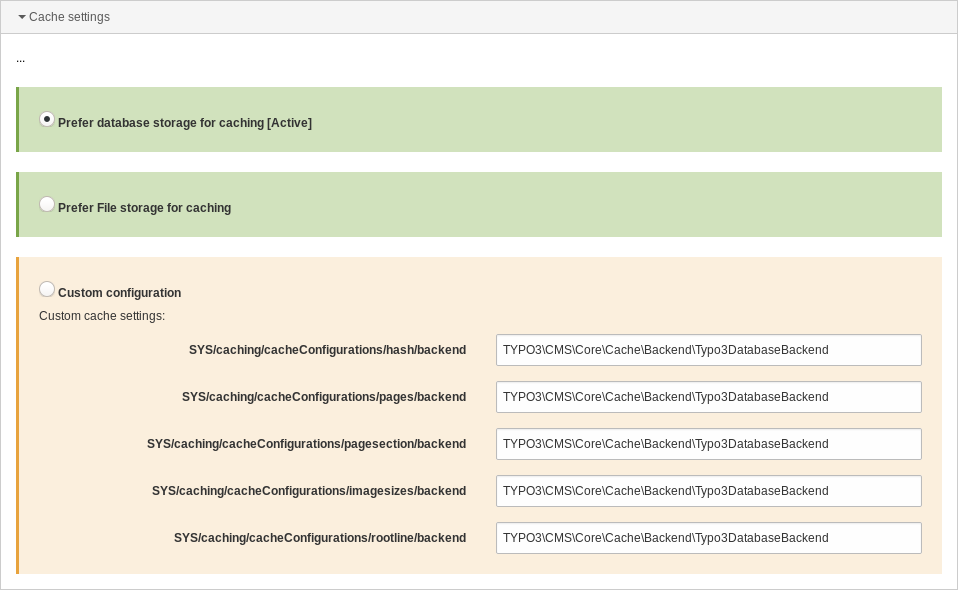
\includegraphics[width=0.60\linewidth]{ChangesForIntegrators/89229-CachePresetForSettingsInMaintenanceArea.png}
	\end{figure}

\end{frame}

% ------------------------------------------------------------------------------
% Feature | 89142 | Create site configuration if page is created on root level

\begin{frame}[fragile]
	\frametitle{Modifiche per integratori}
	\framesubtitle{Configurazione del sito}

	\begin{itemize}
		\item Ogni volta che una nuova pagina è creata a livello root, una configurazione
			standard del sito è generata automaticamente con essa.
		\item Di conseguenza, è possibile configurare velocemente un sito TYPO3 di base.
		\item Le funzionalità di configurazione del sito:

			\begin{itemize}
				\item un identificatore predefinito (es. \texttt{site-42-a1d0c6e83f})
				\item un entry point (es. \texttt{https://example.com/site-42})
				\item una lingua di default (es. \texttt{English})
			\end{itemize}

	\end{itemize}

\end{frame}

% ------------------------------------------------------------------------------
% Feature | 89090 | Reports for conflicting redirects

\begin{frame}[fragile]
	\frametitle{Modifiche per integratori}
	\framesubtitle{Redirect in conflitto (1)}

	\begin{itemize}
		\item Un nuovo comando Symfony è stato inserito per individuare redirect
			in conflitto con url di pagina.
		\item Esegui il comando nella CLI:\newline
			\smaller
				(il parametro opzionale \texttt{-}\texttt{-site} limita la verifica ad un sito specifico)
			\normalsize
	\end{itemize}

	\begin{figure}
		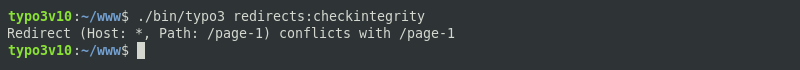
\includegraphics[width=0.90\linewidth]{ChangesForIntegrators/89090a-ReportsForConflictingRedirects.png}
	\end{figure}

	\begin{itemize}
		\item Il comando è disponibile anche come task dello scheduler:
	\end{itemize}

	\begin{figure}
		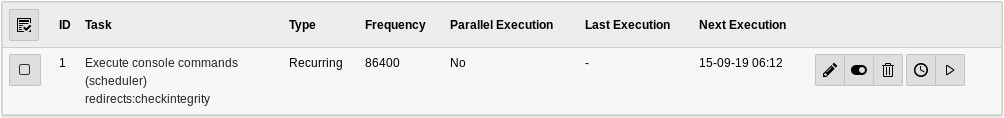
\includegraphics[width=0.90\linewidth]{ChangesForIntegrators/89090b-ReportsForConflictingRedirects.png}
	\end{figure}

\end{frame}

% ------------------------------------------------------------------------------
% Feature | 89090 | Reports for conflicting redirects

\begin{frame}[fragile]
	\frametitle{Modifiche per integratori}
	\framesubtitle{Redirect in conflitto (2)}

	\begin{itemize}
		\item Una lista dei redirect in conflitto individuati può essere esaminata nel modulo Report:
	\end{itemize}

	\begin{figure}
		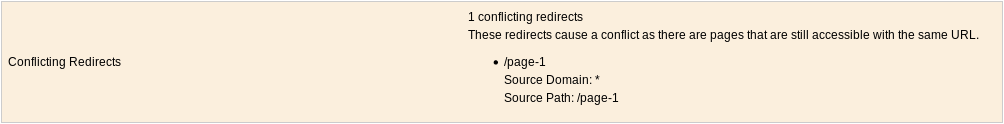
\includegraphics[width=0.90\linewidth]{ChangesForIntegrators/89090c-ReportsForConflictingRedirects.png}
	\end{figure}

	\begin{itemize}
		\item
			\small\textbf{Note:}
				E' necessario avviare nuovamente il comando per svuotare la lista.
				La risoluzione dei problemi (es. rimuovendo il redirect) non pulisce in automatico la lista.
			\normalsize
	\end{itemize}

\end{frame}

% ------------------------------------------------------------------------------
% Feature | 89010 | Introduce Site Configuration for Distribution Packages

\begin{frame}[fragile]
	\frametitle{Modifiche per integratori}
	\framesubtitle{Distribution Packages}

	% decrease font size for code listing
	\lstset{basicstyle=\tiny\ttfamily}

	\begin{itemize}
		\item Le distribuzioni possono contenere file di configurazione del sito.

		\item Crea la directory/file nel distribution package come segue:\newline
			\texttt{Initialisation/Site/<siteIdentifier>/config.yaml}

		\item In modo simile agli assets, che vengono spostati in \texttt{fileadmin/},\newline
			la configurazione del sito viene spostata nella directory \texttt{config/}.

		\item Se la directory di destinazione esiste già, non viene apportata alcuna modifica alla configurazione esistente.
	\end{itemize}

\end{frame}

% ------------------------------------------------------------------------------
% Feature | 88318 | Display Application Context in CLI

\begin{frame}[fragile]
	\frametitle{Modifiche per integratori}
	\framesubtitle{Application Context in CLI}

	\begin{itemize}
		\item L'Application Context corrente è mostrato accanto al numero di versione
			TYPO3 nelle richieste CLI:
	\end{itemize}

	\begin{figure}
		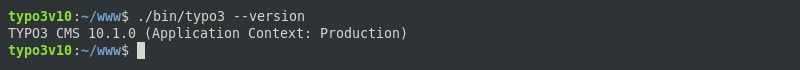
\includegraphics[width=0.90\linewidth]{ChangesForIntegrators/88318-DisplayApplicationContextInCli.png}
	\end{figure}

\end{frame}

% ------------------------------------------------------------------------------
% Feature | 87525 | Add api=1 option in VimeoRenderer

\begin{frame}[fragile]
	\frametitle{Modifiche per integratori}
	\framesubtitle{Vimeo Video Rendering}

	% decrease font size for code listing
	\lstset{basicstyle=\smaller\ttfamily}

	\begin{itemize}
		\item Il parametro \texttt{api=1} nei video Vimeo consente le interazioni API con il lettore video (es. l'aggiunta di pulsanti per controllare il video).
		\item Gli integratori possono ora impostare questo parametro in due modi differenti.

		\begin{itemize}
			\item Usando TypoScript:

\begin{lstlisting}
lib.contentElement.settings.media.additionalConfig.api = 1
\end{lstlisting}

			\item In Fluid usando il Media-ViewHelper:

\begin{lstlisting}
<f:media
  file="{file}"
  alt="{file.properties.alternative}"
  title="{file.properties.title}"
  additionalConfig="{api: 1}"
/>
\end{lstlisting}

		\end{itemize}
	\end{itemize}

\end{frame}

% ------------------------------------------------------------------------------
% Feature | 86670 | Make default action in DragUploader adjustable

\begin{frame}[fragile]
	\frametitle{Modifiche per integratori}
	\framesubtitle{Upload File}

	% decrease font size for code listing
	\lstset{basicstyle=\smaller\ttfamily}

	\begin{itemize}
		\item E' possibile configurare l'azione di default quando viene caricato un file nel modulo "Lista file" utilizzando il drag'n drop.
		\item User TSConfig:

\begin{lstlisting}
# Set default to replace:
options.file_list.uploader.defaultAction = replace

# Set default to rename:
options.file_list.uploader.defaultAction = rename

# Set default to cancel:
options.file_list.uploader.defaultAction = cancel
\end{lstlisting}

	\end{itemize}

\end{frame}

% ------------------------------------------------------------------------------
% Feature | 84250 | Separately enable / disable "Add media by URL" and "Select & upload files"

\begin{frame}[fragile]
	\frametitle{Modifiche per integratori}
	\framesubtitle{Bottoni degli elementi Media}

	% decrease font size for code listing
	\lstset{basicstyle=\tiny\ttfamily}

	\begin{itemize}
		\item I bottoni \textbf{"Add media by URL"} e \textbf{"Select \& upload files"}
			possono essere abilitati/disabilitati indipendentemente l'uno dall'altro.
	\end{itemize}

	\begin{figure}
		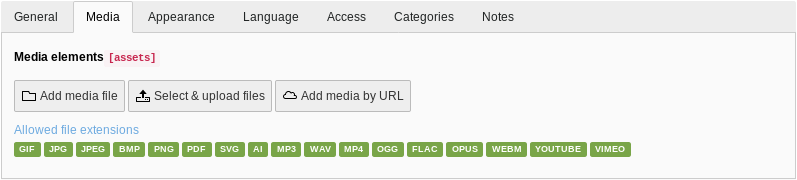
\includegraphics[width=0.75\linewidth]{ChangesForIntegrators/84250-EnableDisableMediaButtons.png}
	\end{figure}

	\begin{itemize}
		\item L'esempio seguente nasconde entrambi i bottoni:

\begin{lstlisting}
$GLOBALS['TCA']['pages']['columns']['media']['config']['appearance'] = [
  'fileUploadAllowed' => false,
  'fileByUrlAllowed' => false,
];
\end{lstlisting}

	\end{itemize}

\end{frame}

% ------------------------------------------------------------------------------
% Feature | 88441 | Show configuration of USER_INT objects in adminpanel

\begin{frame}[fragile]
	\frametitle{Modifiche per integratori}
	\framesubtitle{Admin Panel}

	\begin{itemize}
		\item L'Admin Panel dispone di un nuovo pannello \textbf{USER\_INT} sotto il modulo "Info".
	\end{itemize}

	\begin{figure}
		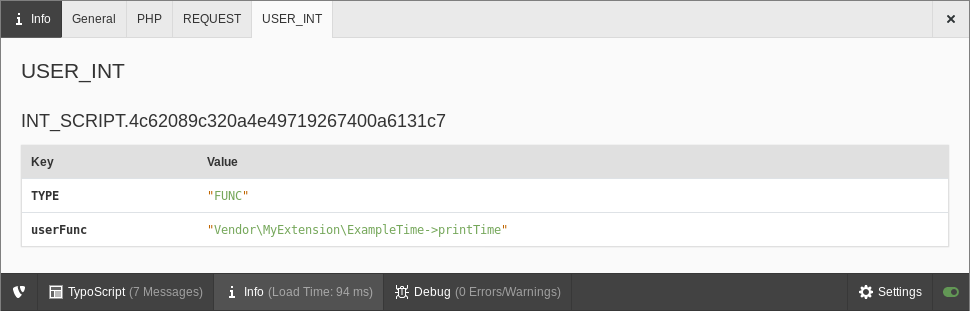
\includegraphics[width=0.90\linewidth]{ChangesForIntegrators/88441-ShowUserIntObjectsInAdminPanel.png}
	\end{figure}

\end{frame}

% ------------------------------------------------------------------------------
